% ===================================================================
%  Week 15 — Sequence Recognition & OCR for DocScan
%  Session 1 of 2: Reading a whole string --- segment-then-classify
%                  vs. end-to-end
% ===================================================================
\documentclass[10pt,aspectratio=169]{beamer}
% ===================================================================
%  Shared Beamer preamble for "Practical Image Processing"
%  English slides. Compile with pdfLaTeX.
% ===================================================================

\usetheme{metropolis}
\usepackage[T1]{fontenc}
\usepackage[utf8]{inputenc}
\usepackage{lmodern}
\usepackage{listings}
\usepackage{tcolorbox}
\usepackage{fontawesome5}
\usepackage{booktabs}
\usepackage{amsmath,amssymb}
\usepackage{tikz}
\usepackage{pgfplots}
\pgfplotsset{compat=1.17}
\usetikzlibrary{arrows.meta,positioning,shapes.geometric,fit,backgrounds,matrix}
\tcbuselibrary{skins,breakable}

% ---- Palette --------------------------------------------------------
\definecolor{coursePrimary}{HTML}{1B4965}   % deep blue
\definecolor{courseAccent}{HTML}{E76F51}    % coral
\definecolor{courseGood}{HTML}{2A9D8F}      % teal
\definecolor{courseBad}{HTML}{C0392B}       % red
\definecolor{courseInfo}{HTML}{2980B9}      % blue
\definecolor{codeBg}{HTML}{F5F6FA}
\definecolor{codeKw}{HTML}{8E44AD}
\definecolor{codeStr}{HTML}{2A9D8F}
\definecolor{codeCom}{HTML}{7F8C8D}

\setbeamercolor{frametitle}{bg=coursePrimary}
\setbeamercolor{progress bar}{fg=courseAccent}
\setbeamercolor{alerted text}{fg=courseAccent}
\metroset{block=fill,sectionpage=progressbar,numbering=fraction}

% ---- Code listings (Python is built into listings) -----------------
\lstdefinestyle{course}{
  backgroundcolor=\color{codeBg},
  basicstyle=\ttfamily\scriptsize,
  keywordstyle=\color{codeKw}\bfseries,
  stringstyle=\color{codeStr},
  commentstyle=\color{codeCom}\itshape,
  numberstyle=\tiny\color{codeCom},
  numbers=left, numbersep=6pt,
  showstringspaces=false, breaklines=true, breakatwhitespace=true,
  tabsize=4, columns=fullflexible,
  frame=single, framesep=4pt, rulecolor=\color{gray!30},
  keepspaces=true, upquote=true, language=Python,
}
\lstset{style=course}
\lstdefinelanguage{bash}{
  keywords={cd,pip,python,venv,source,import}, sensitive=true,
  morecomment=[l]{\#}, morestring=[b]', morestring=[b]",
}

% ---- Reusable callout boxes ----------------------------------------
\newtcolorbox{goodbox}[1][Good practice]{colback=courseGood!8,colframe=courseGood,
  fonttitle=\bfseries,title={\faCheck~#1},boxrule=0.6pt,left=4pt,right=4pt,top=3pt,bottom=3pt}
\newtcolorbox{badbox}[1][Pitfall]{colback=courseBad!8,colframe=courseBad,
  fonttitle=\bfseries,title={\faTimes~#1},boxrule=0.6pt,left=4pt,right=4pt,top=3pt,bottom=3pt}
\newtcolorbox{infobox}[1][Note]{colback=courseInfo!8,colframe=courseInfo,
  fonttitle=\bfseries,title={\faInfoCircle~#1},boxrule=0.6pt,left=4pt,right=4pt,top=3pt,bottom=3pt}
\newtcolorbox{mathbox}[1][Math]{colback=coursePrimary!6,colframe=coursePrimary,
  fonttitle=\bfseries,title={\faCalculator~#1},boxrule=0.6pt,left=4pt,right=4pt,top=3pt,bottom=3pt}

\newcommand{\keyidea}[1]{\begin{alertblock}{Key idea}#1\end{alertblock}}
\newcommand{\term}[1]{\textbf{\color{coursePrimary}#1}}
\newcommand{\code}[1]{\lstinline[basicstyle=\ttfamily\small]|#1|}

% ---- A helper to draw a small pixel grid, cells shaded by value ----
% \pixelgrid{ {10,20,120,200,240}, {30,60,130,180,230}, ... }
\newcommand{\pixelgrid}[1]{%
  \begin{tikzpicture}[font=\scriptsize,scale=0.6]
    \foreach \row [count=\ry] in {#1} {
      \foreach \val [count=\cx] in \row {
        \draw[gray,fill=coursePrimary!8] (\cx,-\ry) rectangle ++(1,-1);
        \node at (\cx+0.5,-\ry-0.5) {\val};
      }
    }
  \end{tikzpicture}}


\title{Sequence Recognition \& OCR}
\subtitle{Week 15 — Session 1: Reading a whole string, not one digit}
\author{Practical Image Processing}
\date{Lecture 15.1 \textbullet\ 60--70 min}

\begin{document}

\maketitle

\begin{frame}{The big idea}
  \begin{columns}[T]
    \begin{column}{0.58\textwidth}
      \begin{itemize}
        \item Week 13: our CNN reads \emph{one} digit at 97\%.
        \item Week 14: object detection \emph{found} the meter and its number window.
        \item \alert{This week:} read the whole numerator --- a \term{string} like \code{018426} --- in one shot.
        \item \textbf{Today (Session 1):} why cutting the string into single digits is fragile, and the end-to-end idea that replaces it.
      \end{itemize}
    \end{column}
    \begin{column}{0.42\textwidth}
      \begin{alertblock}{Where we are heading}
        A reader that takes the cropped meter strip and outputs the \textbf{full number} --- no per-digit scissors. Session 2 builds the CRNN + CTC that make it work.
      \end{alertblock}
    \end{column}
  \end{columns}
\end{frame}

\begin{frame}{Roadmap --- Session 1}\tableofcontents\end{frame}

% ==================================================================
\section{From one digit to a string}
% ==================================================================

\begin{frame}{The DocScan payoff: the whole numerator}
  \begin{columns}[T]
    \begin{column}{0.5\textwidth}
      \begin{center}
      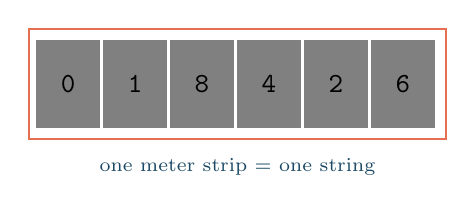
\begin{tikzpicture}[font=\ttfamily]
        \foreach \d [count=\i from 0] in {0,1,8,4,2,6} {
          \draw[fill=coursePrimary!8,gray] (\i*0.85,0) rectangle ++(0.8,1.1);
          \node at (\i*0.85+0.4,0.55) {\d};
        }
        \draw[courseAccent,thick] (-0.1,-0.15) rectangle (5.2,1.25);
        \node[coursePrimary,font=\scriptsize] at (2.55,-0.5) {one meter strip = one string};
      \end{tikzpicture}
      \end{center}
    \end{column}
    \begin{column}{0.5\textwidth}
      \begin{itemize}
        \item DocScan does not want six separate answers --- it wants the reading \code{018426}.
        \item The number of digits \emph{varies} (5, 6, sometimes with a red decimal digit).
        \item Order matters: \code{018426} $\neq$ \code{018462}.
      \end{itemize}
      \keyidea{Our unit of prediction changes: from a single class to an ordered \emph{sequence} of classes.}
    \end{column}
  \end{columns}
\end{frame}

\begin{frame}{The same problem shows up everywhere}
  \begin{columns}[T]
    \begin{column}{0.55\textwidth}
      \begin{itemize}
        \item License plates, receipts, invoices, IDs, handwriting --- all are \emph{sequences} of symbols.
        \item In every case the count is unknown and the symbols can touch or overlap.
        \item ``Read an ordered, variable-length string from an image'' is one of the most common tasks in applied vision.
      \end{itemize}
    \end{column}
    \begin{column}{0.45\textwidth}
      \begin{infobox}[Why meters are a fair proxy]
        A meter numerator is the cleanest version of this task: a single line, fixed alphabet
        (digits), short strings. Master it here, and plates/receipts are the same recipe scaled up.
      \end{infobox}
    \end{column}
  \end{columns}
\end{frame}

\begin{frame}{Two ways to read a string}
  \begin{center}
  \begin{tabular}{@{}p{0.44\textwidth}p{0.44\textwidth}@{}}
    \toprule
    \textbf{Segment-then-classify} & \textbf{End-to-end} \\
    \midrule
    Cut the strip into single digits, then run the Week 13 CNN on each.
      & Feed the whole strip; the model outputs the whole string directly. \\[4pt]
    Needs a reliable \term{segmenter}. & No explicit cutting step. \\[4pt]
    Errors compound across digits. & Trained to optimise the \emph{whole} reading. \\
    \bottomrule
  \end{tabular}
  \end{center}
  \keyidea{Today: see \emph{why} the tidy first option breaks, then meet the second.}
\end{frame}

\begin{frame}{Approach 1: segment-then-classify}
  \begin{center}
  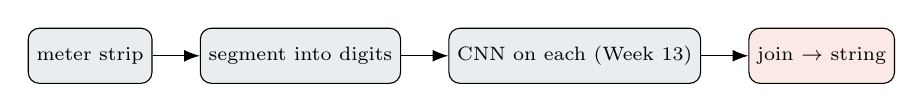
\begin{tikzpicture}[font=\scriptsize,node distance=5mm and 6mm,
      box/.style={draw,rounded corners,fill=coursePrimary!10,minimum height=7mm,inner sep=3pt}]
    \node[box] (strip) {meter strip};
    \node[box,right=of strip] (seg) {segment into digits};
    \node[box,right=of seg] (cls) {CNN on each (Week 13)};
    \node[box,right=of cls,fill=courseAccent!15] (join) {join $\rightarrow$ string};
    \draw[-{Latex[length=2mm]}] (strip)--(seg);
    \draw[-{Latex[length=2mm]}] (seg)--(cls);
    \draw[-{Latex[length=2mm]}] (cls)--(join);
  \end{tikzpicture}
  \end{center}
  \begin{itemize}
    \item Intuitive: we already have a great single-digit classifier.
    \item Each stage is simple in isolation --- classic ``divide and conquer''.
    \item Everything hinges on one brittle assumption: that we can cut cleanly between digits.
  \end{itemize}
\end{frame}

\begin{frame}{Why cutting is hard}
  \begin{columns}[T]
    \begin{column}{0.5\textwidth}
      \begin{itemize}
        \item \term{Touching digits}: no gap to cut on.
        \item \term{Odometer roll-over}: a wheel mid-turn shows \emph{half} of two digits.
        \item Variable spacing, glare, tilt, shadow --- gaps appear and vanish.
        \item How many digits? You must decide \emph{that} too, before reading.
      \end{itemize}
    \end{column}
    \begin{column}{0.5\textwidth}
      \begin{center}
      \begin{tikzpicture}[font=\ttfamily\scriptsize]
        % a half-rolled odometer digit
        \draw[gray,fill=coursePrimary!8] (0,0) rectangle (1,1.4);
        \draw[gray,dashed] (0,0.7)--(1,0.7);
        \node at (0.5,1.05) {7};
        \node at (0.5,0.35) {8};
        \node[coursePrimary,font=\tiny] at (0.5,-0.35) {rolling 7$\to$8};
        \node[courseBad] at (2.2,0.7) {\faQuestion};
        \node[coursePrimary,font=\tiny,align=center] at (2.2,0.2) {which\\ class?};
      \end{tikzpicture}
      \end{center}
      \begin{badbox}[The segmenter is the weak link]
        If the cut is wrong, even a perfect classifier reads garbage.
      \end{badbox}
    \end{column}
  \end{columns}
\end{frame}

\begin{frame}{Errors compound: the multiplication trap}
  Suppose the segmenter is perfect but each digit is read at accuracy $a$. A whole 6-digit
  reading is correct only if \emph{every} digit is correct.
  \begin{mathbox}[Whole-string accuracy]
    $\displaystyle P(\text{string correct}) = a^{L}$ \quad for $L$ independent digits.
  \end{mathbox}
  \begin{center}
  \begin{tabular}{@{}lcccc@{}}
    \toprule
    per-digit $a$ & $L{=}1$ & $L{=}4$ & $L{=}6$ & $L{=}8$ \\
    \midrule
    0.97 & 0.97 & 0.885 & 0.833 & 0.783 \\
    0.99 & 0.99 & 0.961 & 0.941 & 0.923 \\
    \bottomrule
  \end{tabular}
  \end{center}
  \begin{itemize}
    \item Our 97\% digit reader becomes an \textbf{83\%} \emph{string} reader at 6 digits.
    \item And this is the \emph{optimistic} case --- it assumes segmentation never fails.
  \end{itemize}
\end{frame}

\begin{frame}{The two error sources, stacked}
  \begin{center}
  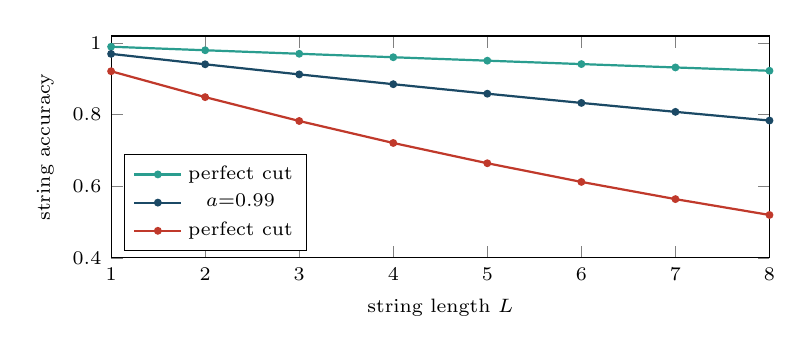
\begin{tikzpicture}[font=\scriptsize]
    \begin{axis}[width=0.82\linewidth,height=4.4cm,
        xlabel={string length $L$},ylabel={string accuracy},
        legend style={font=\scriptsize,at={(0.02,0.03)},anchor=south west},
        tick label style={font=\scriptsize},label style={font=\scriptsize},
        ymin=0.4,ymax=1.02,xmin=1,xmax=8,ytick={0.4,0.6,0.8,1.0}]
      \addplot[courseGood,thick,mark=*,mark size=1pt,samples at={1,...,8}] {0.99^x};
      \addplot[coursePrimary,thick,mark=*,mark size=1pt,samples at={1,...,8}] {0.97^x};
      \addplot[courseBad,thick,mark=*,mark size=1pt,samples at={1,...,8}] {0.97^x*0.95^x};
      \legend{perfect cut, $a{=}0.99$, perfect cut, $a{=}0.97$, +5\% cut error/digit}
    \end{axis}
  \end{tikzpicture}
  \end{center}
  Real pipelines pay for \emph{both} classification and segmentation error --- the red curve falls fast.
\end{frame}

\begin{frame}{So what do we actually want?}
  \begin{itemize}
    \item Avoid committing to cut positions before we understand the image.
    \item Let the reader use \term{context}: a stroke that is ambiguous alone is clear beside its neighbours.
    \item Handle a \emph{variable} number of digits without a separate ``count the digits'' step.
  \end{itemize}
  \begin{goodbox}[The end-to-end promise]
    Read the strip as a whole and output the whole string --- segmentation becomes something the
    model does \emph{implicitly}, if at all.
  \end{goodbox}
\end{frame}

% ==================================================================
\section{The end-to-end view}
% ==================================================================

\begin{frame}{Approach 2: read the strip as a sequence}
  \begin{center}
  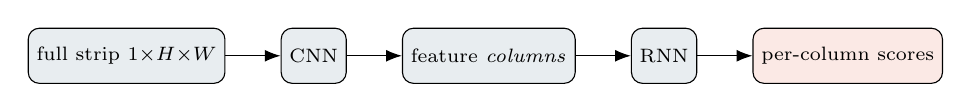
\begin{tikzpicture}[font=\scriptsize,node distance=5mm and 7mm,
      box/.style={draw,rounded corners,fill=coursePrimary!10,minimum height=7mm,inner sep=3pt}]
    \node[box] (strip) {full strip $1{\times}H{\times}W$};
    \node[box,right=of strip] (cnn) {CNN};
    \node[box,right=of cnn] (seq) {feature \emph{columns}};
    \node[box,right=of seq] (rnn) {RNN};
    \node[box,right=of rnn,fill=courseAccent!15] (out) {per-column scores};
    \draw[-{Latex[length=2mm]}] (strip)--(cnn);
    \draw[-{Latex[length=2mm]}] (cnn)--(seq);
    \draw[-{Latex[length=2mm]}] (seq)--(rnn);
    \draw[-{Latex[length=2mm]}] (rnn)--(out);
  \end{tikzpicture}
  \end{center}
  \begin{itemize}
    \item Keep the CNN --- but do \emph{not} pool the width away. Preserve the left-to-right axis.
    \item The CNN turns the strip into a \term{sequence of feature columns}, one per horizontal slice.
    \item That sequence, not a single vector, is what we classify. This is the \term{CRNN} idea (Session 2).
  \end{itemize}
\end{frame}

\begin{frame}{Height collapses, width survives}
  \begin{center}
  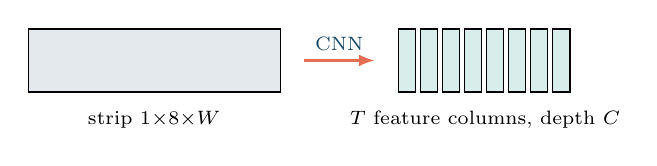
\begin{tikzpicture}[font=\scriptsize]
    % input strip
    \draw[fill=coursePrimary!12] (0,0) rectangle (3.2,0.8);
    \node at (1.6,-0.35) {strip $1{\times}8{\times}W$};
    % arrow
    \draw[-{Latex[length=2mm]},thick,courseAccent] (3.5,0.4)--(4.4,0.4)
      node[midway,above,coursePrimary]{CNN};
    % feature columns
    \foreach \i in {0,...,7} {
      \draw[fill=courseGood!18] (4.7+\i*0.28,0) rectangle ++(0.22,0.8);
    }
    \node at (5.8,-0.35) {$T$ feature columns, depth $C$};
  \end{tikzpicture}
  \end{center}
  \begin{itemize}
    \item Pool the \emph{height} down to 1, but pool the \emph{width} gently (or not at all).
    \item Output: $T$ columns, each a length-$C$ feature vector --- a sequence of length $T$.
    \item Each column ``looks at'' a vertical slice of the strip (its \term{receptive field}).
  \end{itemize}
\end{frame}

\begin{frame}{A column is a soft, overlapping window}
  \begin{columns}[T]
    \begin{column}{0.55\textwidth}
      \begin{itemize}
        \item We never cut the strip. Instead, overlapping columns tile it left to right.
        \item One digit may span \emph{several} columns; a thin digit may share a column with its neighbour.
        \item No column has to contain exactly one digit --- that is the whole point.
      \end{itemize}
    \end{column}
    \begin{column}{0.45\textwidth}
      \begin{center}
      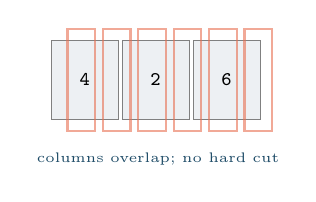
\begin{tikzpicture}[font=\ttfamily\scriptsize]
        \foreach \d [count=\i from 0] in {4,2,6} {
          \draw[gray,fill=coursePrimary!8] (\i*0.9,0) rectangle ++(0.85,1);
          \node at (\i*0.9+0.42,0.5) {\d};
        }
        % overlapping column brackets
        \foreach \x in {0.2,0.65,1.1,1.55,2.0,2.45} {
          \draw[courseAccent,thick,opacity=0.6] (\x,-0.15) rectangle ++(0.35,1.3);
        }
        \node[coursePrimary,font=\tiny] at (1.35,-0.5) {columns overlap; no hard cut};
      \end{tikzpicture}
      \end{center}
    \end{column}
  \end{columns}
\end{frame}

\begin{frame}{No ``count the digits'' step}
  \begin{itemize}
    \item Segment-then-classify must first decide \emph{how many} digits there are --- a separate, error-prone choice.
    \item The end-to-end reader never counts: it emits one label per column, and the collapse rule
          determines the length \emph{implicitly}.
    \item A 4-digit and a 6-digit strip flow through the \emph{same} network unchanged.
  \end{itemize}
  \begin{goodbox}
    Variable length is handled for free --- the output length falls out of decoding, not a preset.
  \end{goodbox}
\end{frame}

\begin{frame}{But now the alignment is unknown}
  \begin{itemize}
    \item The CNN gives $T$ columns (say 12); the true label has $L$ characters (say 6). $T \neq L$.
    \item We do \emph{not} know which columns belong to which digit --- there are no cut marks.
    \item A digit spread over 3 columns will make the RNN say ``4,\,4,\,4'' --- three predictions, one digit.
  \end{itemize}
  \begin{badbox}[The alignment problem]
    We have per-column predictions but an \emph{unaligned}, shorter label. How do we train and decode
    without knowing the column-to-digit mapping?
  \end{badbox}
  \keyidea{This is exactly what \term{CTC} solves --- the star of Session 2.}
\end{frame}

\begin{frame}{A tiny taste of the fix (no maths yet)}
  \begin{columns}[T]
    \begin{column}{0.55\textwidth}
      \begin{itemize}
        \item Let the model also emit a special \term{blank} symbol \code{-} meaning ``no new character here''.
        \item Read off the raw per-column output, then apply two rules:
        \begin{enumerate}
          \item collapse \emph{repeats}, then
          \item drop \emph{blanks}.
        \end{enumerate}
      \end{itemize}
    \end{column}
    \begin{column}{0.45\textwidth}
      \begin{mathbox}[Collapse example]
        raw:\ \ \code{4\,4\,-\,2\,2\,2\,-\,6}\\[2pt]
        collapse repeats:\ \code{4\,-\,2\,-\,6}\\[2pt]
        drop blanks:\ \ \code{4\,2\,6}
      \end{mathbox}
    \end{column}
  \end{columns}
  \vspace{2pt}
  The blank lets a repeated digit (\code{4\,4} for \emph{two} fours) survive --- we will make this precise next time.
\end{frame}

\begin{frame}{Why the RNN, not just the CNN?}
  \begin{itemize}
    \item A CNN column sees only a local slice --- good for strokes, blind to long context.
    \item An \term{RNN} passes information \emph{along} the sequence, left to right (and right to left).
    \item So each column's decision can use its neighbours: ``this smudge is a 1 because a 0 sits beside it.''
  \end{itemize}
  \begin{goodbox}
    CNN = \emph{what does this slice look like}; RNN = \emph{what makes sense given the slices around it}.
  \end{goodbox}
\end{frame}

\begin{frame}{The name: CRNN}
  \begin{center}
  
\begin{tikzpicture}[font=\scriptsize,node distance=4mm and 7mm,
      box/.style={draw,rounded corners,fill=coursePrimary!10,minimum height=7mm,inner sep=3pt,align=center}]
    \node[box] (c) {\textbf{C}NN\\[-1pt]\tiny feature columns};
    \node[box,right=of c] (r) {\textbf{R}NN\\[-1pt]\tiny context along width};
    \node[box,right=of r,fill=courseAccent!15] (t) {\textbf{transcription}\\[-1pt]\tiny CTC decode};
    \draw[-{Latex[length=2mm]}] (c)--(r);
    \draw[-{Latex[length=2mm]}] (r)--(t);
  \end{tikzpicture}
  \end{center}
  \begin{itemize}
    \item \term{CRNN} = Convolutional Recurrent Neural Network: the standard OCR backbone.
    \item CNN extracts, RNN contextualises, a transcription layer (CTC) turns columns into the final string.
    \item One network, trained end to end, from strip image to reading --- no segmenter to tune.
  \end{itemize}
\end{frame}

\begin{frame}{Where this sits in DocScan}
  \begin{center}
  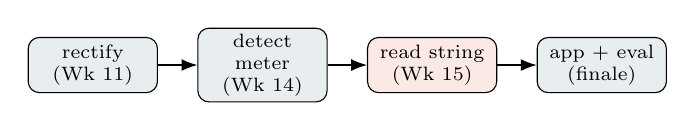
\begin{tikzpicture}[font=\scriptsize,node distance=4mm and 5mm,
      box/.style={draw,rounded corners,fill=coursePrimary!10,minimum height=7mm,inner sep=2pt,text width=15mm,align=center}]
    \node[box] (w11) {rectify\\ (Wk 11)};
    \node[box,right=of w11] (w14) {detect meter\\ (Wk 14)};
    \node[box,right=of w14,fill=courseAccent!15] (w15) {read string\\ (Wk 15)};
    \node[box,right=of w15] (w16) {app + eval\\ (finale)};
    \draw[-{Latex[length=2mm]}] (w11)--(w14);
    \draw[-{Latex[length=2mm]}] (w14)--(w15);
    \draw[-{Latex[length=2mm]}] (w15)--(w16);
  \end{tikzpicture}
  \end{center}
  \begin{itemize}
    \item Weeks 1--11 gave us a clean, rectified crop; Week 14 located the number window.
    \item This week reads it --- the last \emph{algorithmic} piece before the capstone finale.
  \end{itemize}
\end{frame}

% ==================================================================
\section{In-class exercise}
% ==================================================================

\begin{frame}{\faPen~In-class exercise (10 min)}
  \begin{infobox}[Reason about reading a whole string]
  \end{infobox}
  \begin{enumerate}
    \item A digit reader is 98\% accurate \emph{per digit}, cuts are perfect. What is its expected
          \emph{whole-string} accuracy on a 5-digit meter?
    \item Give two physical reasons a meter strip cannot be reliably cut between digits.
    \item The CNN emits 10 feature columns for a 4-digit reading. Is $T>L$, $T=L$, or $T<L$ here,
          and why is that the comfortable case?
    \item Apply ``collapse repeats, then drop blanks'' to the raw output
          \code{9\,9\,-\,-\,0\,-\,0\,0}. What string results?
  \end{enumerate}
\end{frame}

\begin{frame}{\faPen~Debrief}
  \begin{itemize}
    \item (1) $0.98^{5} \approx 0.904$ --- about \textbf{90\%}, already a 10-point drop from the per-digit number.
    \item (2) Touching digits (no gap) and odometer roll-over (a wheel showing half of two digits);
          also glare/tilt that erase or invent gaps.
    \item (3) $T{=}10>L{=}4$: more slots than characters, so blanks can absorb the slack --- CTC needs $T\ge L$.
    \item (4) collapse \code{9\,9}$\to$\code{9}, \code{0\,0}$\to$\code{0}: \code{9\,-\,0\,-\,0}; drop blanks $\Rightarrow$ \code{900}.
  \end{itemize}
  \keyidea{You can already reason about string accuracy, why cutting fails, and the collapse rule --- the CTC machinery next time makes it exact.}
\end{frame}

% ==================================================================
\section{Wrap-up}
% ==================================================================

\begin{frame}{Common pitfalls (today's ideas)}
  \begin{badbox}[Watch out]
    \begin{itemize}
      \item Reporting the \emph{per-digit} accuracy as if it were the reading accuracy.
      \item Trusting a segmenter on touching or rolling digits --- the classic field failure.
      \item Pooling the \emph{width} away in the CNN: you destroy the very axis you need to read along.
      \item Forgetting that $T$ (columns) and $L$ (characters) are different, unaligned quantities.
    \end{itemize}
  \end{badbox}
\end{frame}

\begin{frame}{Good habits}
  \begin{goodbox}
    \begin{itemize}
      \item Always quote \emph{string}-level and \emph{character}-level accuracy, never just per-digit.
      \item Prefer end-to-end reading when digits touch, roll, or vary in count.
      \item Keep the width axis intact through the CNN; collapse only the height.
      \item Think in ``columns'', not ``cut-out digits'' --- overlap is a feature, not a bug.
    \end{itemize}
  \end{goodbox}
\end{frame}

\begin{frame}{What you can already do}
  \begin{itemize}
    \item Explain why segment-then-classify multiplies errors and breaks on real meters.
    \item Describe the end-to-end alternative: CNN feature columns $\rightarrow$ RNN $\rightarrow$ transcription.
    \item State the alignment problem ($T \neq L$) and the collapse-repeats-then-drop-blanks rule.
    \item Place the string reader inside the full DocScan pipeline.
  \end{itemize}
\end{frame}

\begin{frame}{Next session}
  \begin{alertblock}{Session 2 --- CRNN + CTC, made precise}
    \begin{itemize}
      \item The CRNN in detail: CNN $\rightarrow$ map-to-sequence $\rightarrow$ BiLSTM $\rightarrow$ per-column scores.
      \item \term{CTC loss}: summing over \emph{all} alignments so we can train without cut marks.
      \item Decoding: greedy (best path) vs.\ beam search, and the collapse rule made exact.
      \item Evaluating a reader with \term{edit distance}, CER, and whole-string accuracy --- then code it and ship the meter-string reader.
    \end{itemize}
  \end{alertblock}
  \emph{Bring today's ``columns, not cuts'' picture --- next time we teach the network to align itself.}
\end{frame}

\begin{frame}[standout]
  Read the string, don't cut it into digits.\\[4pt]
  \normalsize Today: why cutting fails and the end-to-end idea. Next: CRNN + CTC make it real.
\end{frame}

\end{document}
